\section{软件变更获取}\label{software-diff-extract}

进行软件变更分析首先需要获取软件变更,一般情况下,变更获取算法可基于纯文本或基于树结构进行分析。在对 AOSP 进行分析的场景下,借助 git 这一版本控制管理中的对象文件可以更好地获取变更信息——git 可获取的变更信息大致被分为两类,分别是变更文件元数据信息以及具体文本差异。本节讨论了两类方法在该场景下的优劣,并给出了适当的变更获取算法。

\subsection{基于纯文本的变更获取算法}

获取软件变更的最简便方法是使用基于纯文本的变更获取算法。

Webb Miller 等人提出了一段基于文本的文件对比程序\cite{SPAE-1985-AFileComparisonProgram}。文章中给出了简洁的文件对比程序项目源码。Muhammad Asaduzzaman 等人提出了一种基于文本的语言无关文本差异获取算法\cite{ICSM-2013-AsaduzzamanRSP}。算法通过建立 “候选列表” 猜测源文件到目标文件的可能映射,使用摘要算法确定对应关系。因此,分别获取两个版本中的所有文件并进行比较是一种获取变更差异的可行方案。

由于 AOSP 中所有仓库都使用 git 作为版本控制系统,而 git 中使用二进制对象存储了相邻两个版本之间的软件变更情况(文件内容增加与删除情况),且 git 中实现过 Myers、Minimal、Patience 以及 Histogram 四种文本差异算法\cite{Nugroho_2019},所以任意两个版本之间的软件变更都可以通过 git 获取。但需要注意的是,git 作为通用版本控制系统,其中用于得出两版本间差异的算法是与语言无关的文本差异算法,不存在对于特定文本文件类型优化的情况。也就是说,基于 git 内部数据结构实现的变更获取算法必定是基于纯文本的。然而,上文提及的纯文本变更获取算法存在着下述问题:

\begin{itemize}
    \item 基于纯文本的变更获取算法很难进行空间与时间复杂度的权衡。
    \item 现有基于纯文本的变更获取算法在程序设计方面较为简洁,很难提升程序的可扩展性。
    \item 基于纯文本的变更获取算法忽视了源文件中的代码结构。
\end{itemize}

基于纯文本的变更差异分析仅仅能够获取方法名,但对于方法的形参获取存在一定的困难。这种困难主要是程序设计上的。因此放弃 AST 选用纯文本意味着放弃了具有足够表达能力的工具,也同时意味着获取方法形参类型代码片段必定具备相当的复杂性。

\subsection{基于树的变更获取算法}

软件分析并不需要将项目中所有文件都纳入分析范围。一个项目中可能存在相当大部分的文件与项目核心功能无关。这些无关文件的修改并不会对项目核心功能造成影响。更进一步地,仅仅考虑核心代码文件而忽视诸如文本文件、配置文件、测试文件等无关文件,可能会在降低分析任务量、提高分析速度的同时,不丧失对项目核心功能变更的把控。相较于基于纯文本的变更获取算法,基于树的变更获取算法不再忽视源文件中的结构,可以获取更细粒度的变更信息。

Jean-Remy Falleri 等人提出了一种细粒度的源代码差异分析算法,并实现了名为 gumTree 的变更获取工具\cite{DBLP:conf/kbse/FalleriMBMM14}。该算法作为一种语言相关的算法,不再以 “行” 作为最小单元,而是以抽象语法树为基础,以抽象语法树叶子节点作为最小单元。但该工具的实现并没有在其建立的树结构与抽象语法树之间建立联系,这使得该工具专注于变更节点,而难以获取变更节点的父子节点信息。KaiFeng Huang 等人基于 Jean-Remy Falleri 的工作提出了一种可控粒度(表达式、语句、方法)的源代码差异算法,并实现了名为 CLDIFF 的工具\cite{10.1145/3238147.3238219}。但该工具与能够作为代码库被用户直接使用的 gumTree 不同,CLDIFF 系统较为庞大,同时也并不支持灵活的应用场景,这也就意味着将 CLDIFF 从文章描述的场景迁移到 AOSP 下需要一定的工作。

\subsection{变更信息获取方法的选取}

上文主要讨论了两类变更获取算法,不同变更获取算法所能获取的变更信息种类不同——基于文本的变更获取算法通常以 “行” 为构成文件的基本单元,所以此类算法仅可以给出源文件到目标文件的 “新增行” 与 “删减行” 的列表;而基于树的变更获取算法可以通过设置 “抽象语法树节点”、“表达式”、“语句” 等不同粒度来满足分析需要。

对于本文所设计的软件变更分析系统而言,软件变更获取是进行后续分析的前置条件。因此在设计该模块整体架构与所使用的算法时,必须考虑模块间分析与模块内分析的具体输入。

由于 AOSP 中各仓库均使用了 git 作为版本控制系统,所以本文所设计的软件变更分析系统可以通过 git 中的二进制对象获取 AOSP 下某仓库研发流程的所有关键信息。“文件” 是 git 中重要的基本单元,通过 git 可以获得诸如 “暂存区”、“提交”、“差异入口” 等常用于项目开发与静态分析的一类与 “文件” 有关的信息。同时,以 Ninja 构建系统为例,在 AOSP 构建过程当中,\ref{aosp-introduction}中提出的单一构建过程概念描述了多个输入文件(节点)到多个输出文件(节点)的映射,不难得出 “文件” 是 Ninja 构建系统中的重要概念。且根据 Ninja 源代码可知,Ninja 只有在首次构建时才必定执行完整构建过程。构建产物仍然存在于输出路径之下时,Ninja 在再次构建前会比较 “源文件与构建产物的时间戳”,以此忽略不必要的构建过程。

以 git 版本控制系统为例,在给定项目中,单一文件可能在整个研发流程中存在各种各样的软件变更,且该类变更无法仅通过 “文件” 级别信息获取。因此不满足于 git 提供的 “文件” 级别信息、获取更细粒度的变更差异是必要的。AOSP Frameworks 下绝大多数源代码文件都是由 Java 编写的,剩余文件由字符串 xml 文件、配置文件、文本文件等无关文件组成,这类无关文件在项目中与项目核心功能无关,且此类文件的修改并不会对项目核心功能造成影响。而对于 Java 程序设计语言而言,类作为 “一等公民” 被广泛使用,类中声明或实现的方法描述了类的可能行为。

综上所述,在本文所设计的软件变更分析系统中,我综合使用了两类变更获取算法:

\begin{itemize}
    \item 文件级别:使用基于文本的变更获取算法,如图\ref{fig:git-alg}所示分析给定软件在两个版本之间存在变更的文件入口。通过这些文件入口,可以获得文件路径、文件最后修改者、增加或删减的字符串等信息。以文件作为变更信息的维度之一,不仅可以通过 git 获取大量信息,还能在后续分析中基于已有的 Ninja 代码框架进一步开发。
    \item 方法级别:使用基于树的变更获取算法\ref{alg:get-method-name},获得包括但不限于给定软件在两个版本之间遭到修改的方法名等信息。以方法作为变更信息的维度之一,不仅可以使用基于树的变更获取算法高效获取细粒度差异,还可以在后续的模块内部分析中获得受变更影响的方法。

\end{itemize}

\begin{figure}
    \centering
    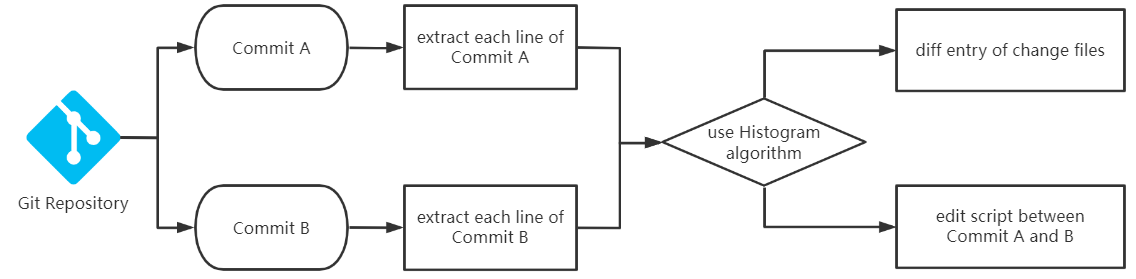
\includegraphics[width=.8\textwidth]{figures/git-alg.png}
    \caption{使用 git 获取两版本间变更文件}
    \label{fig:git-alg}
\end{figure}

\vskip 13.8pt
\renewcommand{\thealgorithm}{1}
    \begin{algorithm}
        \caption{方法名获取算法}
        \begin{algorithmic}[1]
            \Require 差异文件入口到文本差异的映射 $M$
            \Ensure 差异文件信息 $Info$
            \State initialize $l$ as a list
            \For{$(entry, script) \Leftarrow M$}
                \State $tree \Leftarrow entry.node$
                \If{tree's ancestor exists "MethodDeclaration"}
                    \State $l \Leftarrow tree$
                \EndIf
            \EndFor
            \For{$node \in l$}
                \State get $methodName$ by node's ancestor
                \State $Info \Leftarrow methodName$
            \EndFor
            \State \Return $Info$
        \end{algorithmic}
        \label{alg:get-method-name}
    \end{algorithm}
    \vskip 13.8pt
